\section{Introduction and Motivation}
\label{sec:intro}
%% ============================================================

Standard transformers (GPT) compute a sequence of \emph{additive} residual updates:
each block reads the current hidden state, computes an attention output and an MLP
output, and adds them to the state.
The updates are independent across blocks, and each block is specialised by training
to contribute a different transformation.

Energy-based models (EGPTs) were proposed as an alternative in which each block
performs one step of gradient descent on a shared energy function $E(h)$.
The intuition is that the sequence of blocks then implements an iterative inference
procedure, converging toward a low-energy configuration.
This design has several theoretical virtues: it provides a variational interpretation
of inference, enables test-time compute scaling by adding extra recurrence steps, and
may encourage convergence toward a stable attractor rather than accumulating noise.

In practice, the original EGPT formulation is substantially less compute-efficient than GPT.
The $V{=}K$ constraint (using keys as values, so that attention output lies on the key
manifold) introduces a structural bottleneck: the $4.4\times$ FLOPs overhead of an EGPT
over a comparable GPT yields only GPT-equivalent accuracy.

This paper is a systematic ablation study that traces a path from the original EGPT to
a family of architectures, \textbf{EGrad} and \textbf{EDesc}, that match or exceed GPT at
the same compute budget.
The key insight is not architectural complexity: it is a \emph{single change to the output
rule} of the energy attention heads.

\paragraph{Roadmap.}
\begin{itemize}
  \item Section~\ref{sec:architectures}: Forward-pass equations for all variants (GPT, EGPT, Mixed, EGrad, EDesc).
  \item Section~\ref{sec:egpt_gap}: Diagnosing the compute gap between EGPT and GPT.
  \item Section~\ref{sec:probes}: Mechanistic probes: Helmholtz decomposition, layer similarity, and weight merging.
  \item Section~\ref{sec:mixed}: Mixed heads close the gap.
  \item Section~\ref{sec:output_rule}: The output-rule change that crosses the GPT frontier.
  \item Section~\ref{sec:scaling}: Scaling EGrad/EDesc to 400M parameters confirms the advantage.
\end{itemize}

\begin{figure}[h]
  \centering
  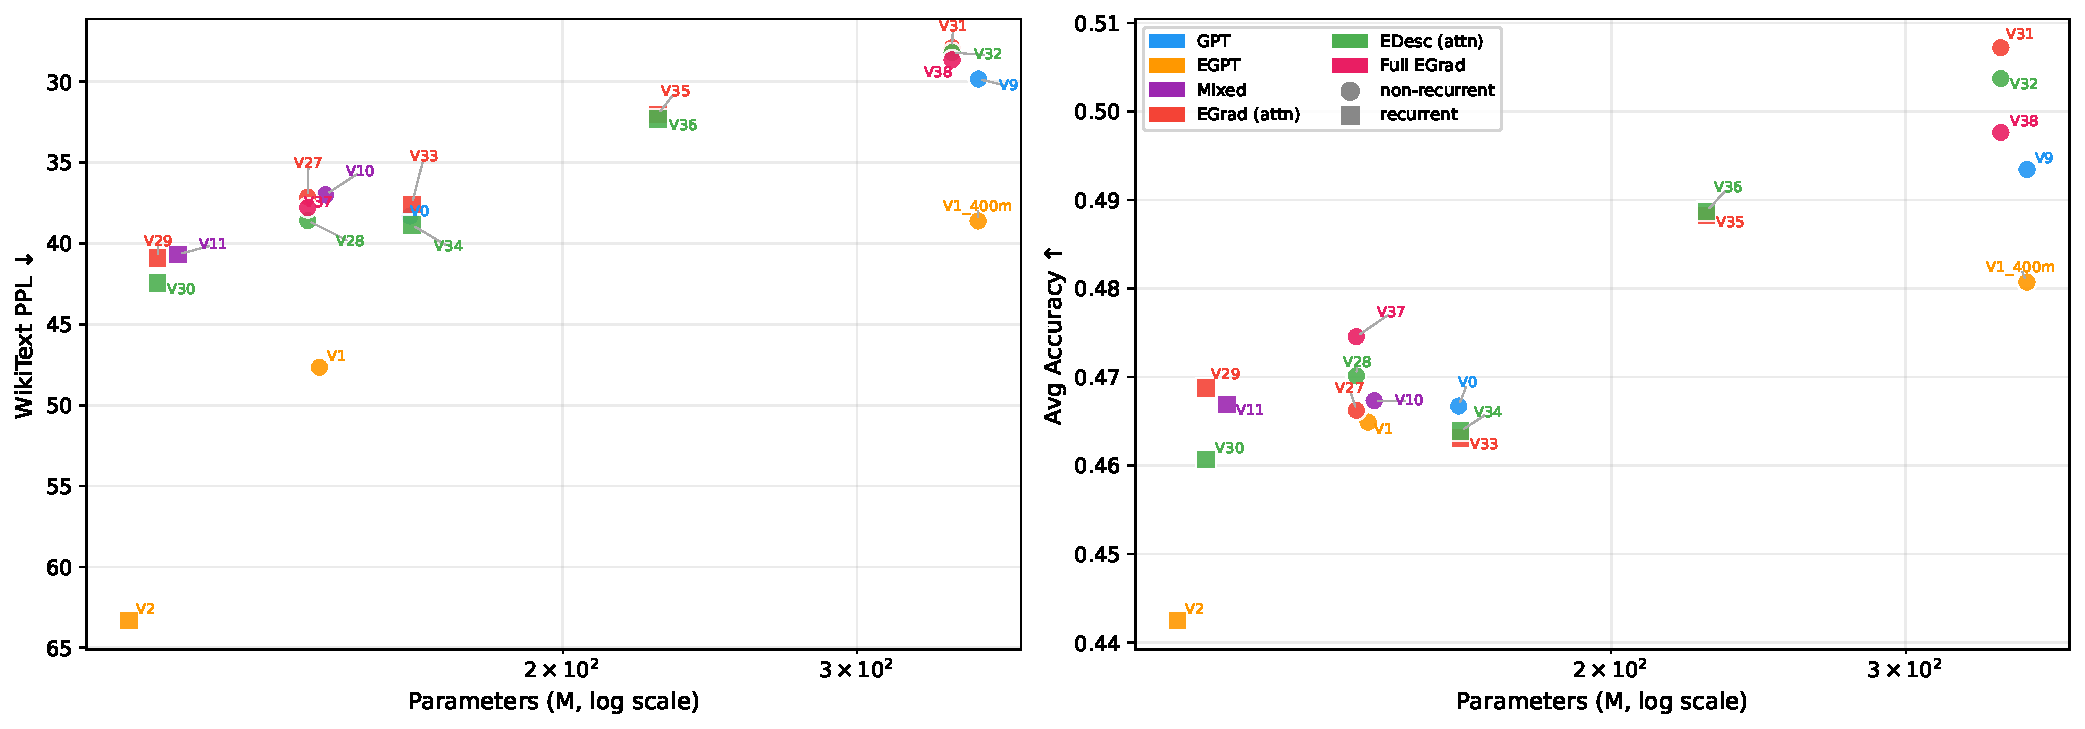
\includegraphics[width=\textwidth]{../results/multi-block-ablation/plots/headline_ppl_acc_vs_params.pdf}
  \caption{Headline results --- PPL and average accuracy vs.\ parameter count (log scale).
    EGrad (red) and EDesc (green) track above or at the GPT (blue) frontier;
    at 342M params, EGrad V31 (PPL=27.9, 50.7\%) outperforms V9 GPT (PPL=29.8, 48.6\%).
    Squares = recurrent (weight-shared) models; circles = non-recurrent.
    Mixed (grey; plain MixedHead runs) excluded from this view ---
    see Appendix for comparison.}
  \label{fig:headline_params}
\end{figure}

\begin{figure}[h]
  \centering
  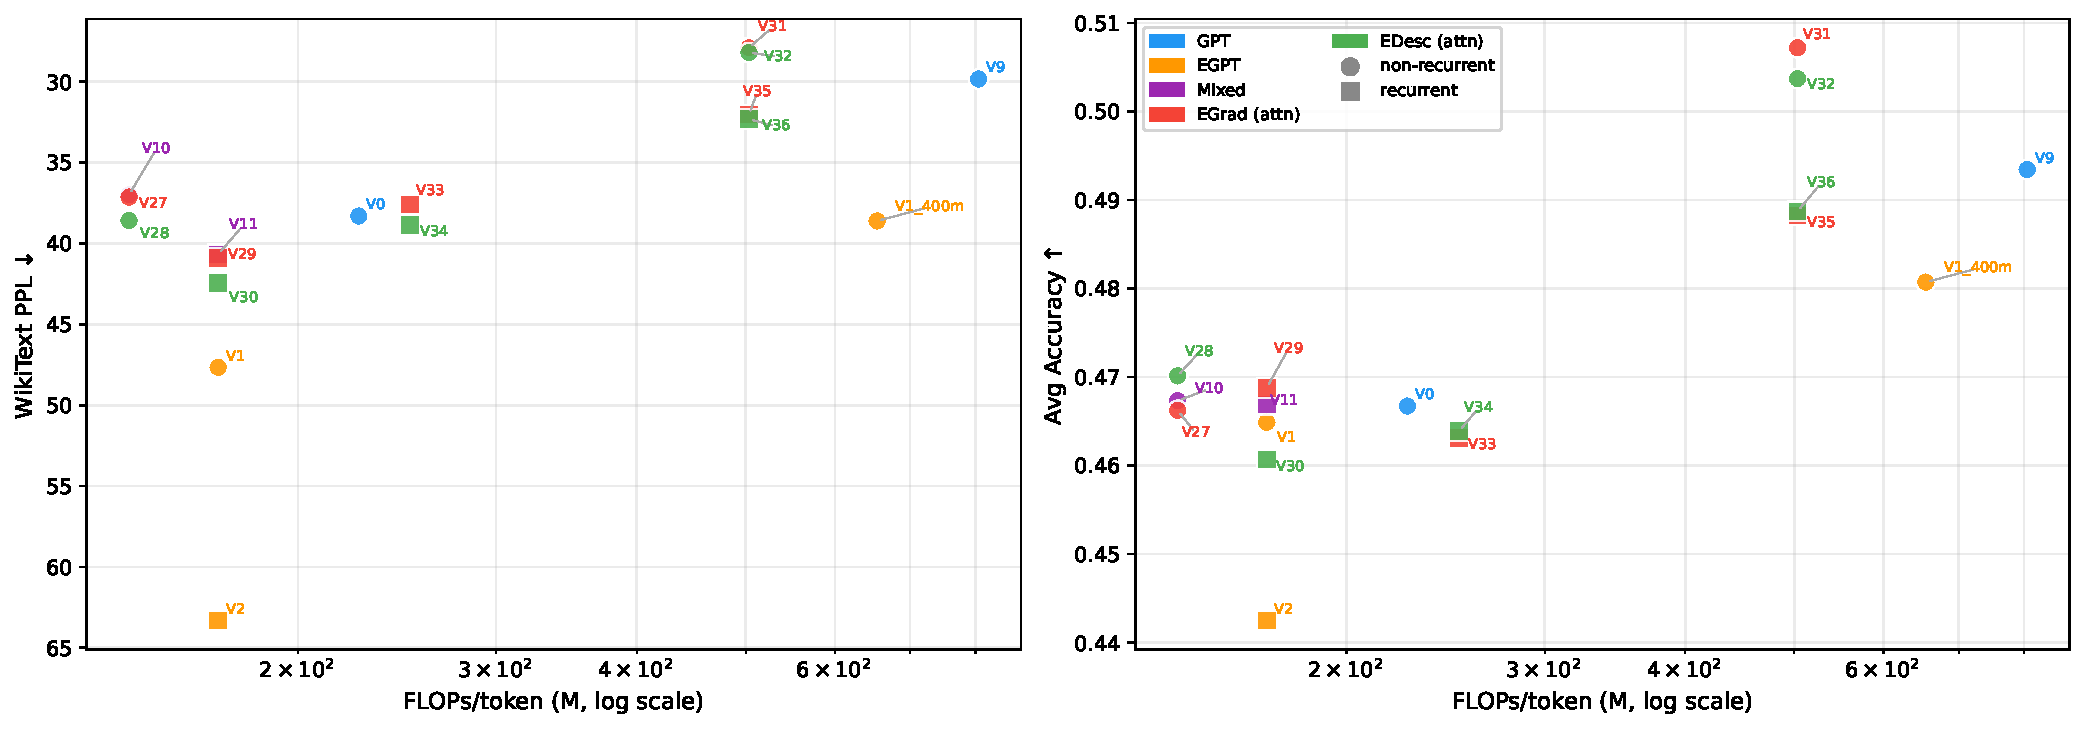
\includegraphics[width=\textwidth]{../results/multi-block-ablation/plots/headline_ppl_acc_vs_flops.pdf}
  \caption{Headline results --- PPL and average accuracy vs.\ FLOPs/token (log scale).
    EGrad/EDesc (red/green) match or exceed GPT (blue) at every compute budget tested.
    At 503 MFLOPs/tok, EGrad V31 strictly dominates V9 GPT on both axes.
    Recurrent models (squares) trade unique-parameter count for FLOPs efficiency.}
  \label{fig:headline_flops}
\end{figure}

%% ============================================================
